\chapter{Methodology for evaluation of dynamic performance}
\label{chap3}

\section{General work flow}
Figure \ref{fig:workflow} illustrates the general work flow for the evaluation of dynamic performance. The first step is to create mesh models in Rhino with different combinations of geometric parameters. Then, the mesh models are exported in Abaqus for modal analysis. As a next step, modal parameters (natural frequencies, modal masses, modes shapes) from modal analysis are extracted to solve the response time history of the floor under footfall excitation via modal superposition. Once the response from each mode is available, post-processing of the response will be conducted based on the procedure presented by the evaluation guideline. Finally, the post-processed response will be compared with the acceptance criteria and a conclusion about the vibration level can be drawn.

\begin{figure}[H]
\centering
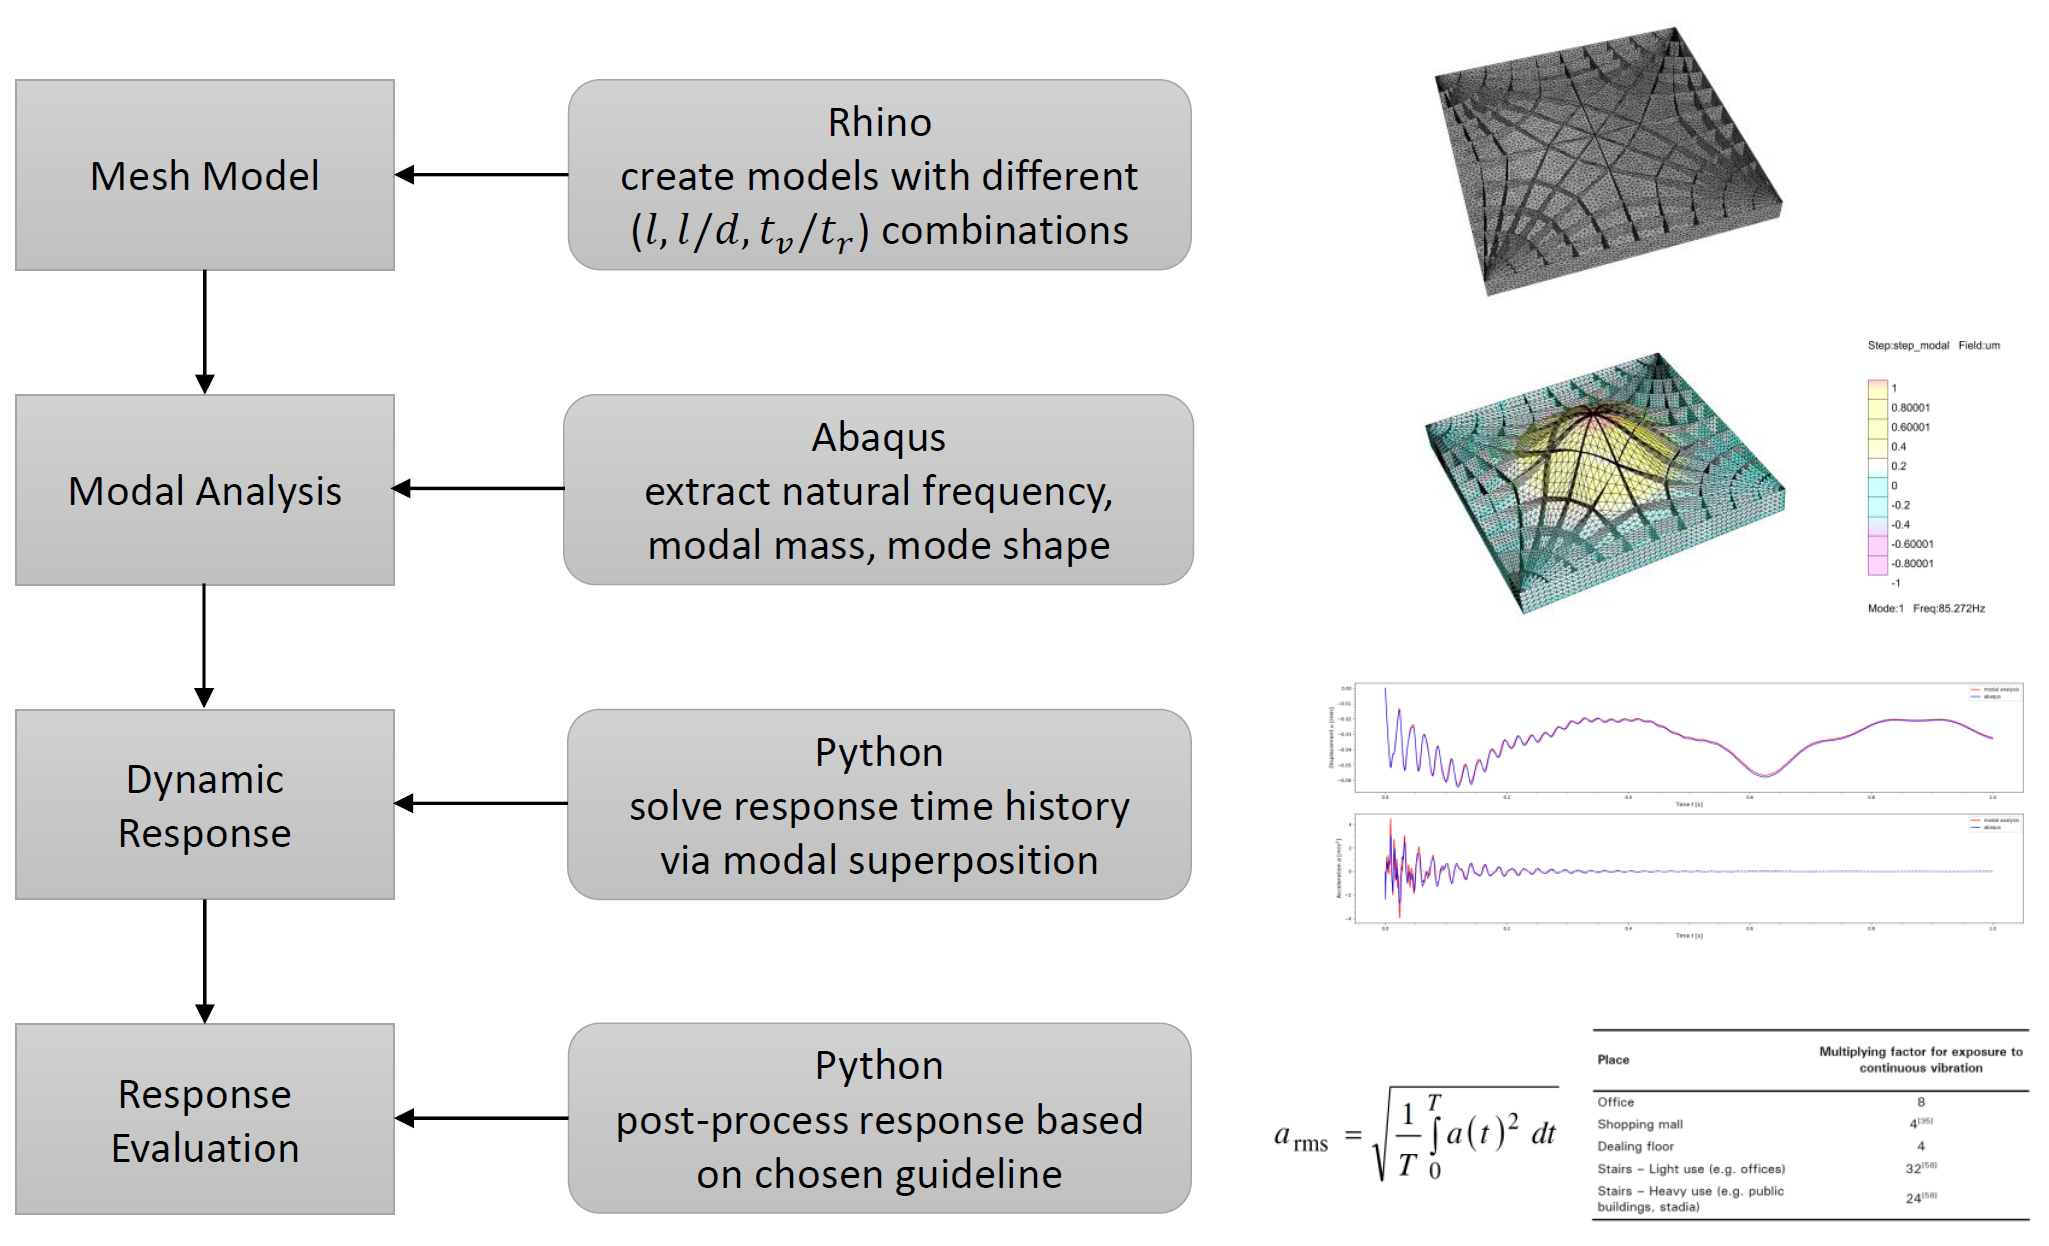
\includegraphics[width=1.0\textwidth]{workflow}
\caption{Work flow for evaluation of vibration}
\label{fig:workflow}
\end{figure}

\section{Modeling}
\subsection{Mesh model generation}
Three geometrical parameters are considered important to outline the geometry of a floor if the pattern of ribs is given: the span $l$, span/depth ratio $l/d$ and vault/ribs thickness ratio $t_v/t_r$. Some assumptions are made to avoid unnecessary complexity: the floor has a square form in plane; the vault has a constant thickness everywhere, so do the ribs, although vault and ribs can show different thicknesses; the top of the neutral surface of the vault is 5cm under the upper bound of the floor, this value does not change with the span. The three parameters have the following values covering realistic ranges in practical use as well as reasonably exaggerated ranges for research reasons:
\begin{align*}
    l&=[5,6,7,8,9,10]\quad[m]\\
    l/d&=[10,12.5,15,17.5,20]\quad[-]\\
    t_v/t_r&=[0.1,0.5,1,2,5,10]\quad[-]
\end{align*}

The geometry of the vault and ribs is form-found based on TNA and created with COMPAS\_TNA package. The span and depth of the floor is easy to scale, but the pattern of ribs not. To ensure that floors with different spans have similar ribs density (similar panel size surrounded by ribs), the numbers of ribs in both circular and radial directions are scaled in proportion to the span. The thickness of vault and ribs is given in form of thickness ratio under the condition that the floor mass equals to a constant value, no matter how the ratio varies. The floor mass is set to be 40\% of the mass of a solid rectangular one with the same outer geometry. If the total volume of the floor $v$, the area of the vault $a_v$ and ribs $a_r$, and thickness ratio $\gamma = t_v/t_r$ are known, the thickness of ribs and vault can be determined by
\begin{align}
    t_r &= \frac{v}{\gamma a_v+a_r}\\
    t_v &= \gamma t_r
\end{align}

Figure \ref{fig:mehs_models} shows the mesh models of floors with constant $l/d=15$ and all above listed spans. The combination of the three parameters will generate 180 models for analysis.

\begin{figure}[H]
\begin{subfigure}[b]{.48\textwidth}
  \centering
  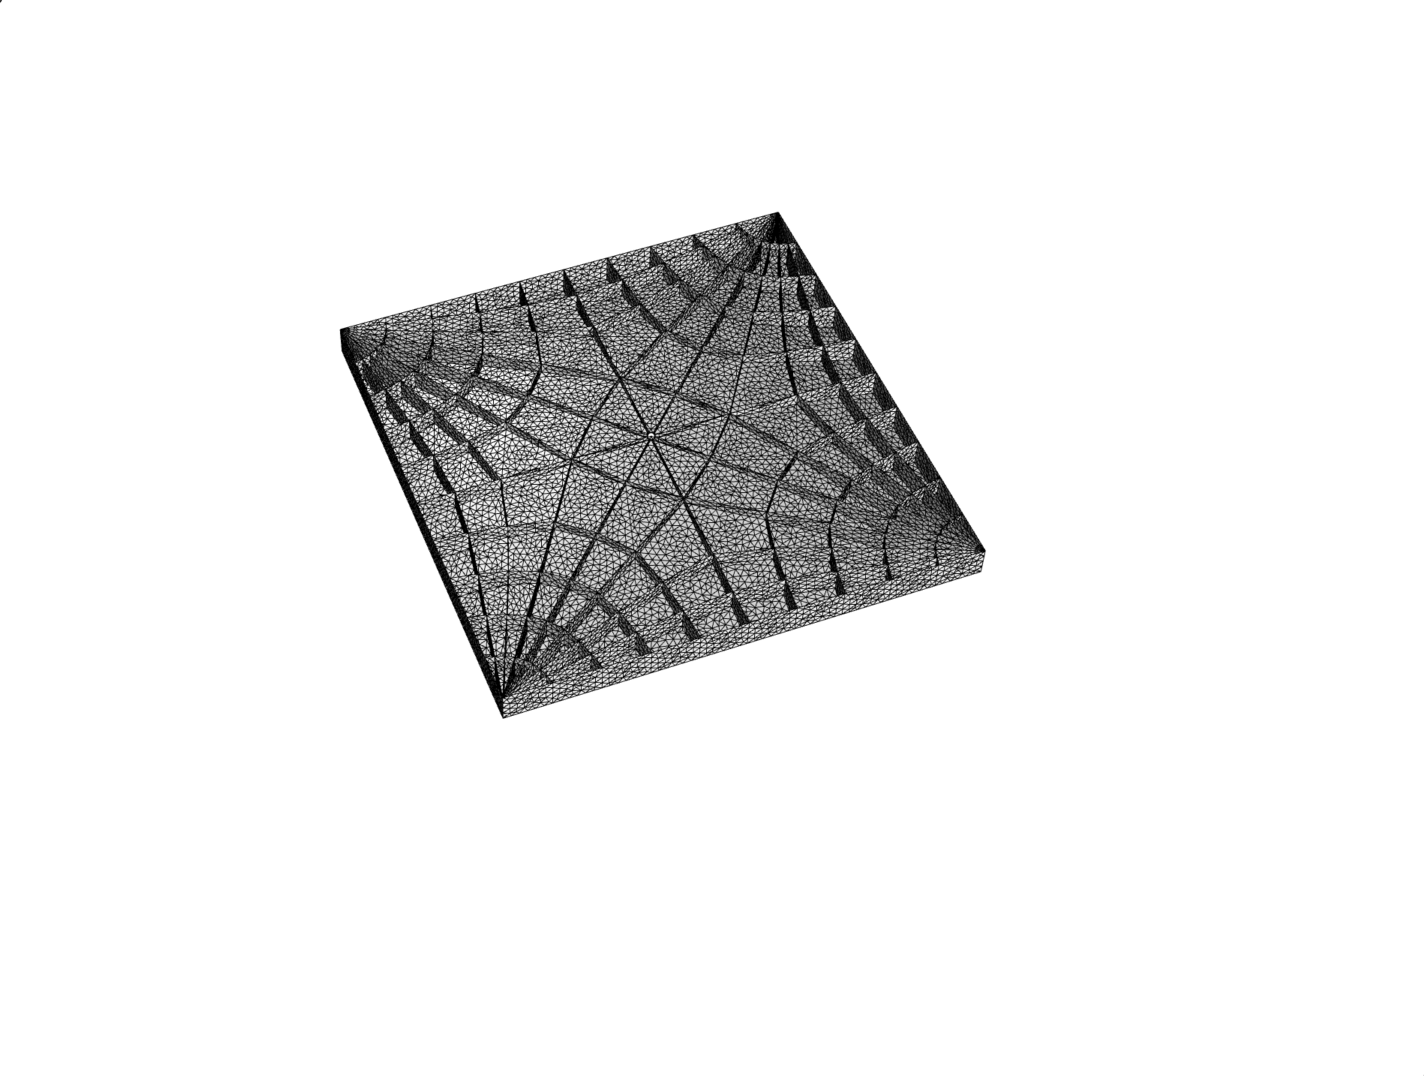
\includegraphics[width=.95\linewidth]{span5}
  \caption{span=5m}
\end{subfigure}
~
\begin{subfigure}[b]{.48\textwidth}
  \centering
  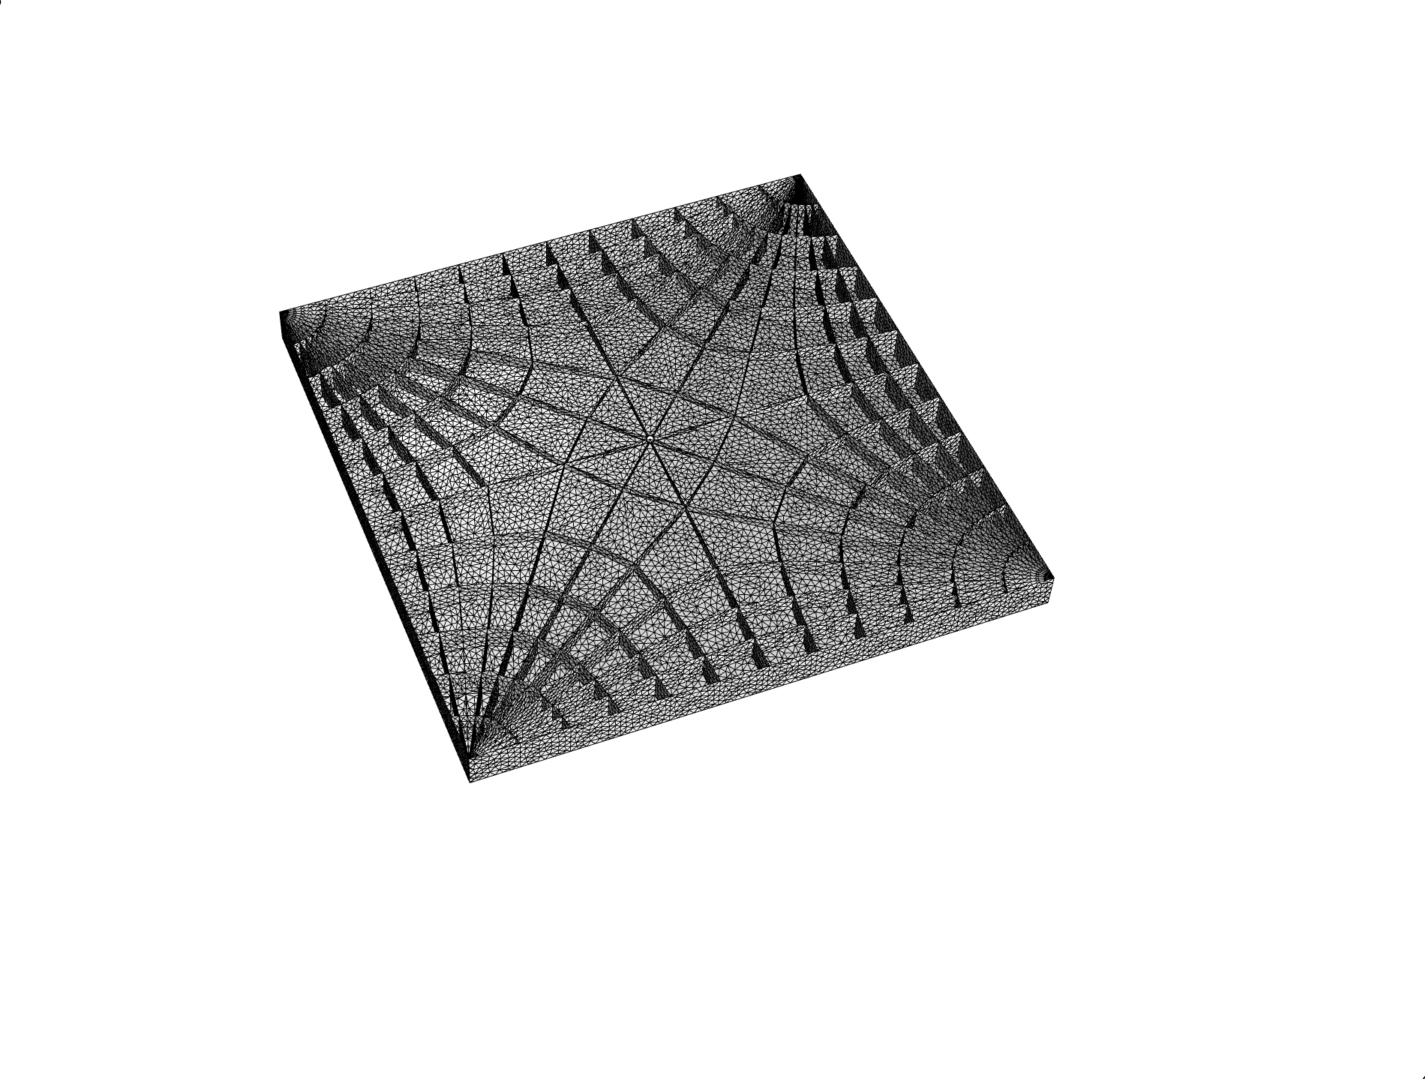
\includegraphics[width=.95\linewidth]{span6}
  \caption{span=6m}
\end{subfigure}

\begin{subfigure}[b]{.48\textwidth}
  \centering
  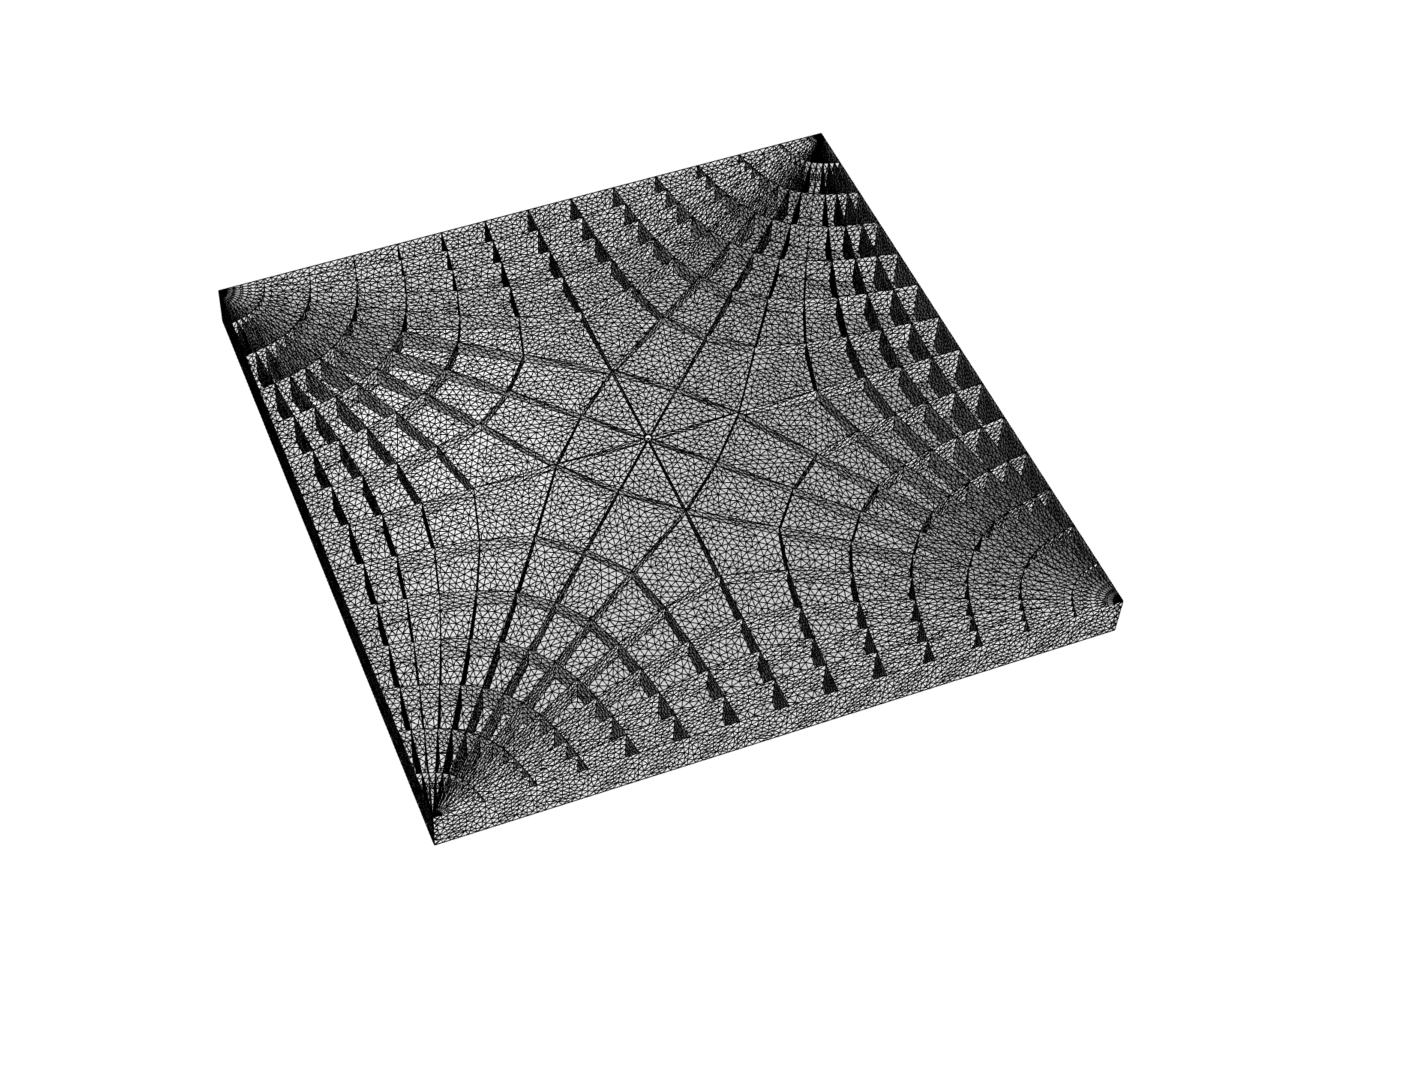
\includegraphics[width=.95\linewidth]{span7}
  \caption{span=7m}
\end{subfigure}
~
\begin{subfigure}[b]{.48\textwidth}
  \centering
  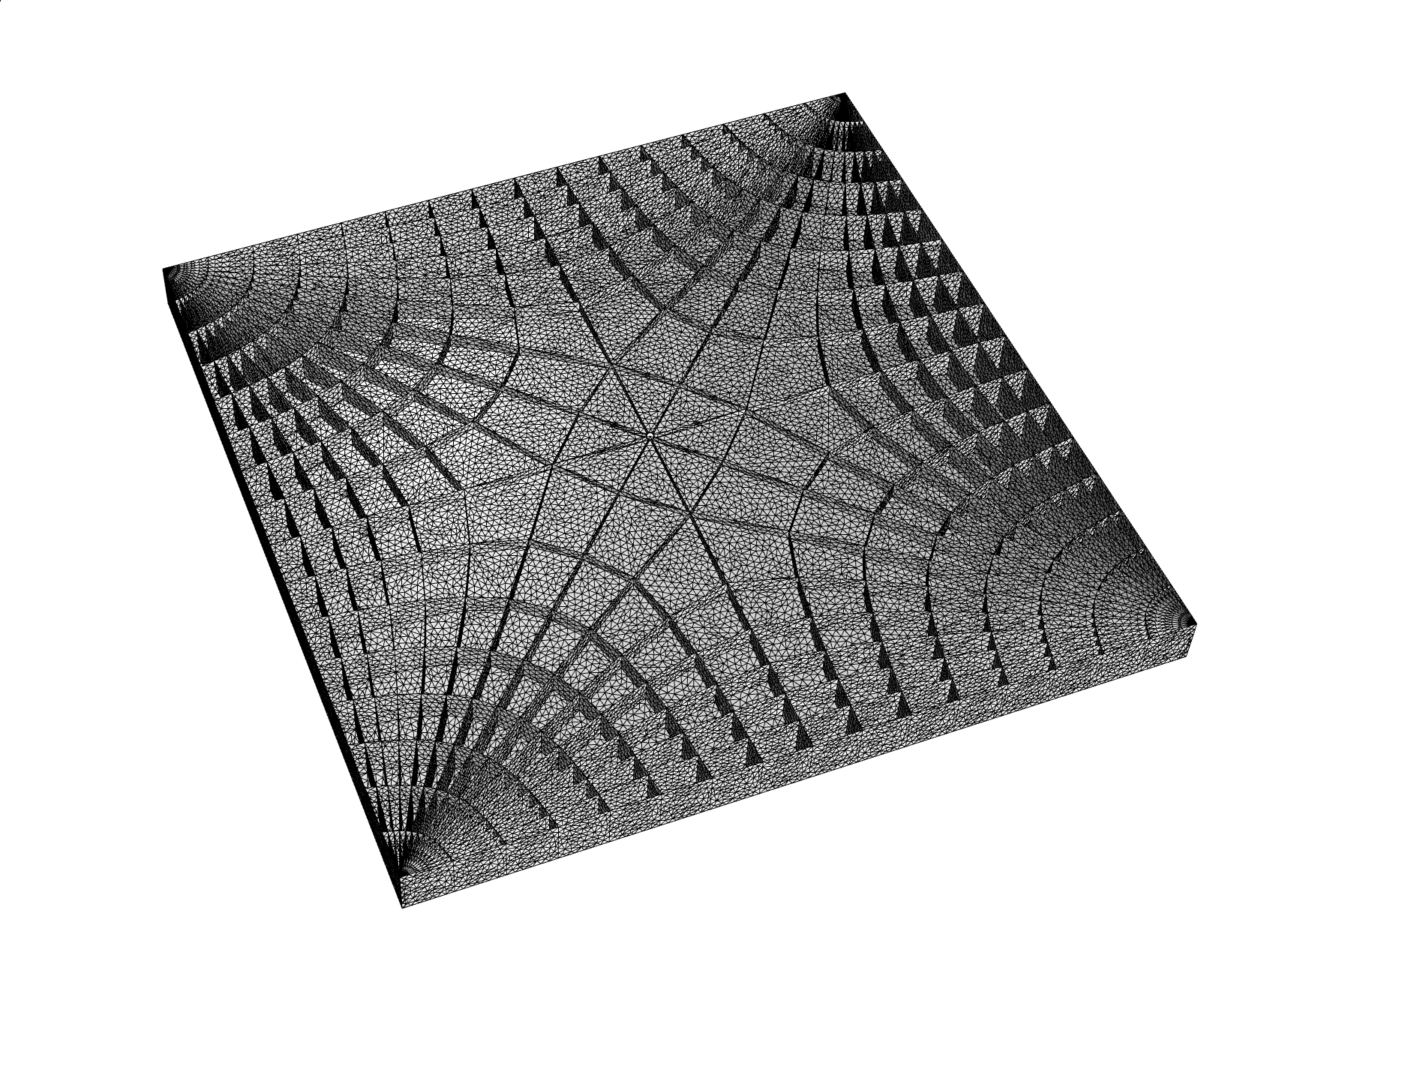
\includegraphics[width=.95\linewidth]{span8}
  \caption{span=8m}
\end{subfigure}

\begin{subfigure}[b]{.48\textwidth}
  \centering
  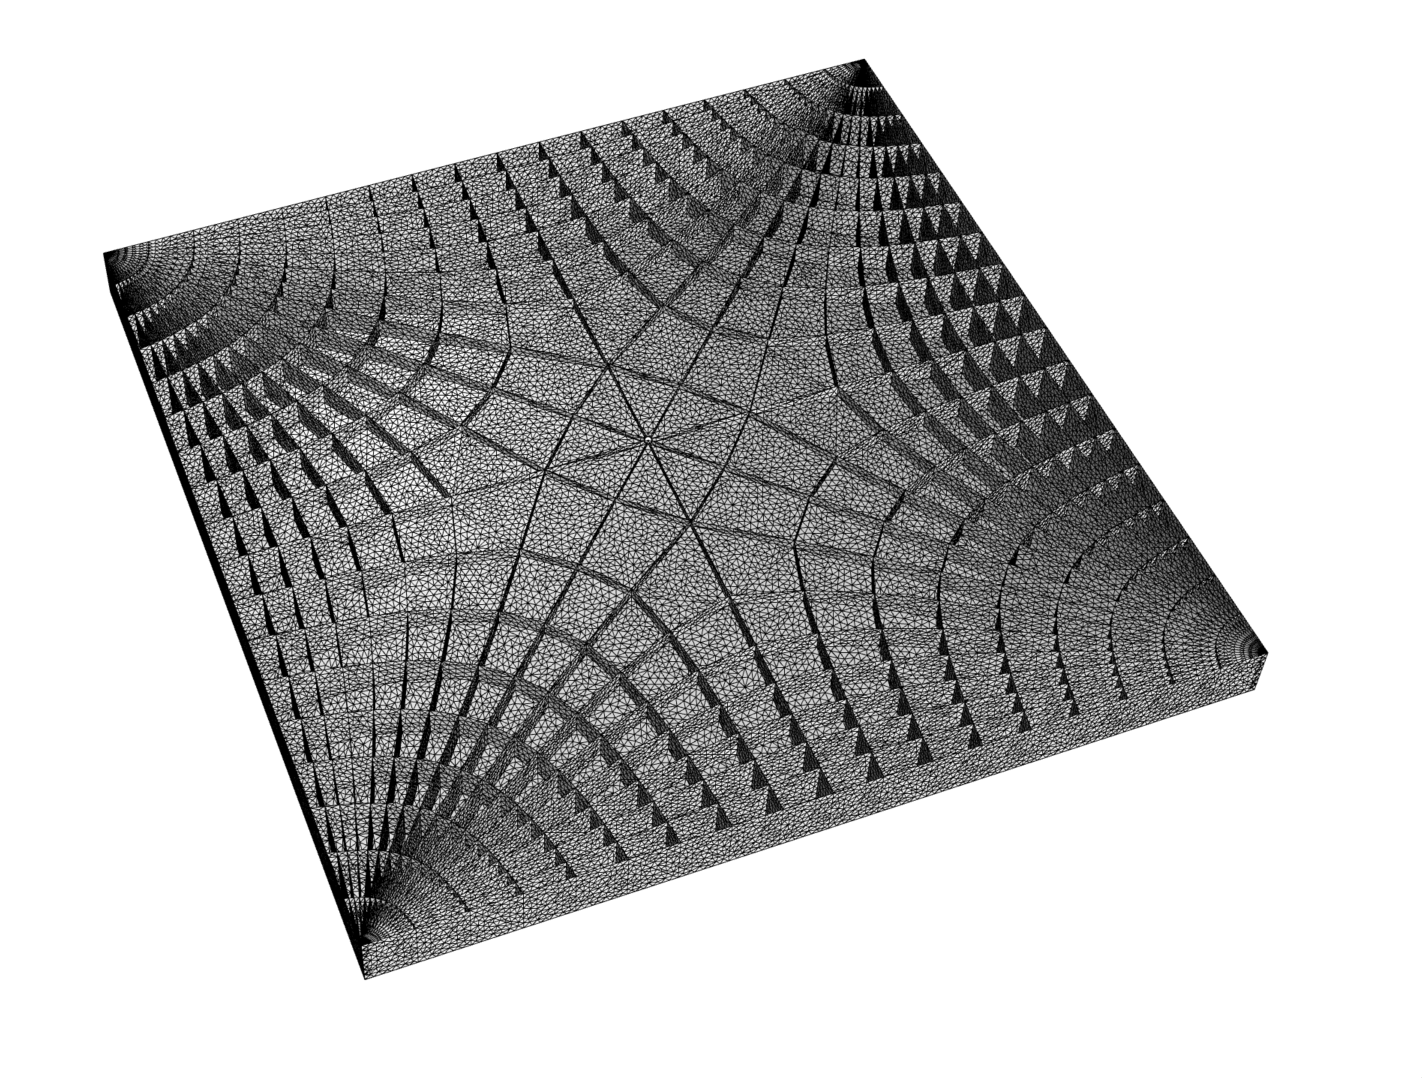
\includegraphics[width=.95\linewidth]{span9}
  \caption{span=9m}
\end{subfigure}
~
\begin{subfigure}[b]{.48\textwidth}
  \centering
  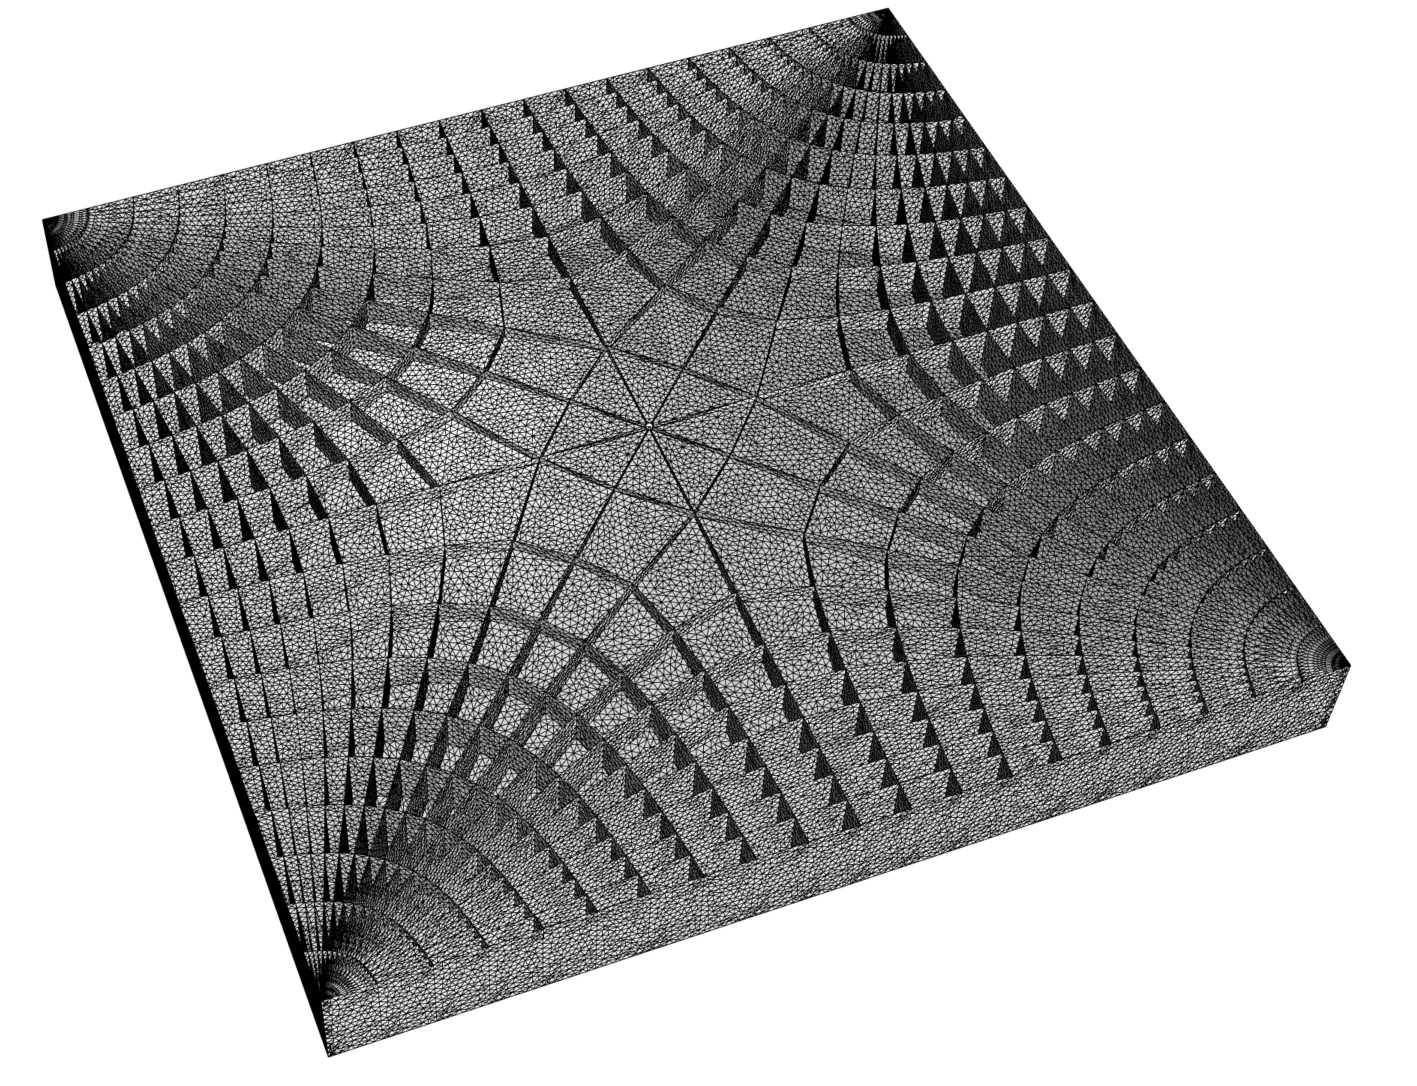
\includegraphics[width=.95\linewidth]{span10}
  \caption{span=10m}
\end{subfigure}

\caption{Mesh models with different spans}
\label{fig:mehs_models}
\end{figure}

\subsection{Material of choice}
The floor will be made of fiber-reinforced concrete. The density and Poisson's ratio are set to be 2400 kg/m$^3$ and 0.2 respectively, the same as common engineering use. The Young's modulus,nevertheless, should take a higher value for a dynamic process. A dynamic Young's modulus of 38 GPa is proposed by SCI P354 for normal weight concrete, irrespective of the actual concrete class. An isotropic elastic behavior of the concrete is assumed for this floor, as the excess of the tensile strength of concrete for such a compression dominate floor is unlikely during human-induced vibration, and the potential anisotropic behavior that may be introduced by rebars in normal reinforced concrete is also excluded here.

\subsection{Structural considerations}
Shell elements will be provided to represent the floor mesh. Given that the floor is considered to be resting without connection constraining rotation on the four supporting edges, these have been considered as lines of pinned nodes, as in vibration the strains are not large enough to overcome the friction \cite{smith2007design}, even though the floor may have roller boundary conditions for static cases. The structural frame that would support the floor element in the construction setting is not considered as part of the modeling. A damping ratio of 3\% is assumed for fully fitted out and furnished floors in normal use \cite{smith2007design}. The beneficial influence of office partitions on the stiffness and additional masses of furniture and finishing is conservatively not considered.

\subsection{Footfall loading}
The excitation point and response point should be chosen to produce the maximum response of the floor. In most cases the two points will represent the same point. Theoretically, it should be checked for every point defined in the finite element analysis. In practice, however, only the points that correspond to the maximum amplitudes for each mode need to be checked \cite{smith2007design}. As the first mode whose vibration shape has its peak in the middle dominates the response, the footfall excitation is presumed to act on the middle point of the floor. 

Continuous footfall excitation is uncommon, but it is representative of the worst possible loading scenario for a given forcing function. The forcing function from a walking activity is assumed to perfectly periodic and can be represented by the sum of four harmonic Fourier series in time history:
\begin{equation}
P(t)=W\left[1+\sum_h\alpha_h \sin(2\pi h f_\mathrm{p} t + \phi_h)\right]
\label{eqn:footfall_SCI}
\end{equation}
where:\par
\makebox[1.5cm]{$W$}  is the weight of an average person\par
\makebox[1.5cm]{$h$}  is the harmonic mode number\par
\makebox[1.5cm]{$\alpha_h$} is the dynamic coefficient for mode $h$\par
\makebox[1.5cm]{$f_\mathrm{p}$} is the pacing frequency\par
\makebox[1.5cm]{$\phi_h$} is the phase angle\par
\noindent
These Fourier coefficients can be extracted from table \ref{tab:fourier coeff}.

{
\renewcommand{\arraystretch}{1.2}
\begin{table}[H]
\centering
\caption{Fourier coefficients for walking activities}
\label{tab:fourier coeff}
\begin{tabular}{cccc}
\Xhline{2\arrayrulewidth}
\textbf{harmonic} & \textbf{pace frequency} & \textbf{dynamic coefficient} & \textbf{phase angle} \\
$\boldsymbol{h}$    & $\boldsymbol{hf_p}$ \textbf{(Hz)}  & $\boldsymbol{\alpha_h}$        & $\boldsymbol{\phi_h}$ \\ \Xhline{2\arrayrulewidth}
1                 & 1.8 to 2.2              & 0.436($hf_p$-0.95)           & 0                    \\
2                 & 3.6 to 4.4              & 0.006($hf_p$+12.3)           & $-\pi/2$                    \\
3                 & 5.4 to 6.6              & 0.007($hf_p$+5.2)            & $\pi$                    \\
4                 & 7.2 to 8.8              & 0.007($hf_p$+2.0)            & $\pi/2$                    \\ \Xhline{2\arrayrulewidth}
\end{tabular}
\end{table}
}
\noindent
A pace frequency of 2 Hz is adopted for analysis, figure \ref{fig:footfall} plots the footfall load time history for one walking cycle (two pace periods, 1 second). The peak value can be ca. 70\% higher than the average.
\begin{figure}[H]
\centering
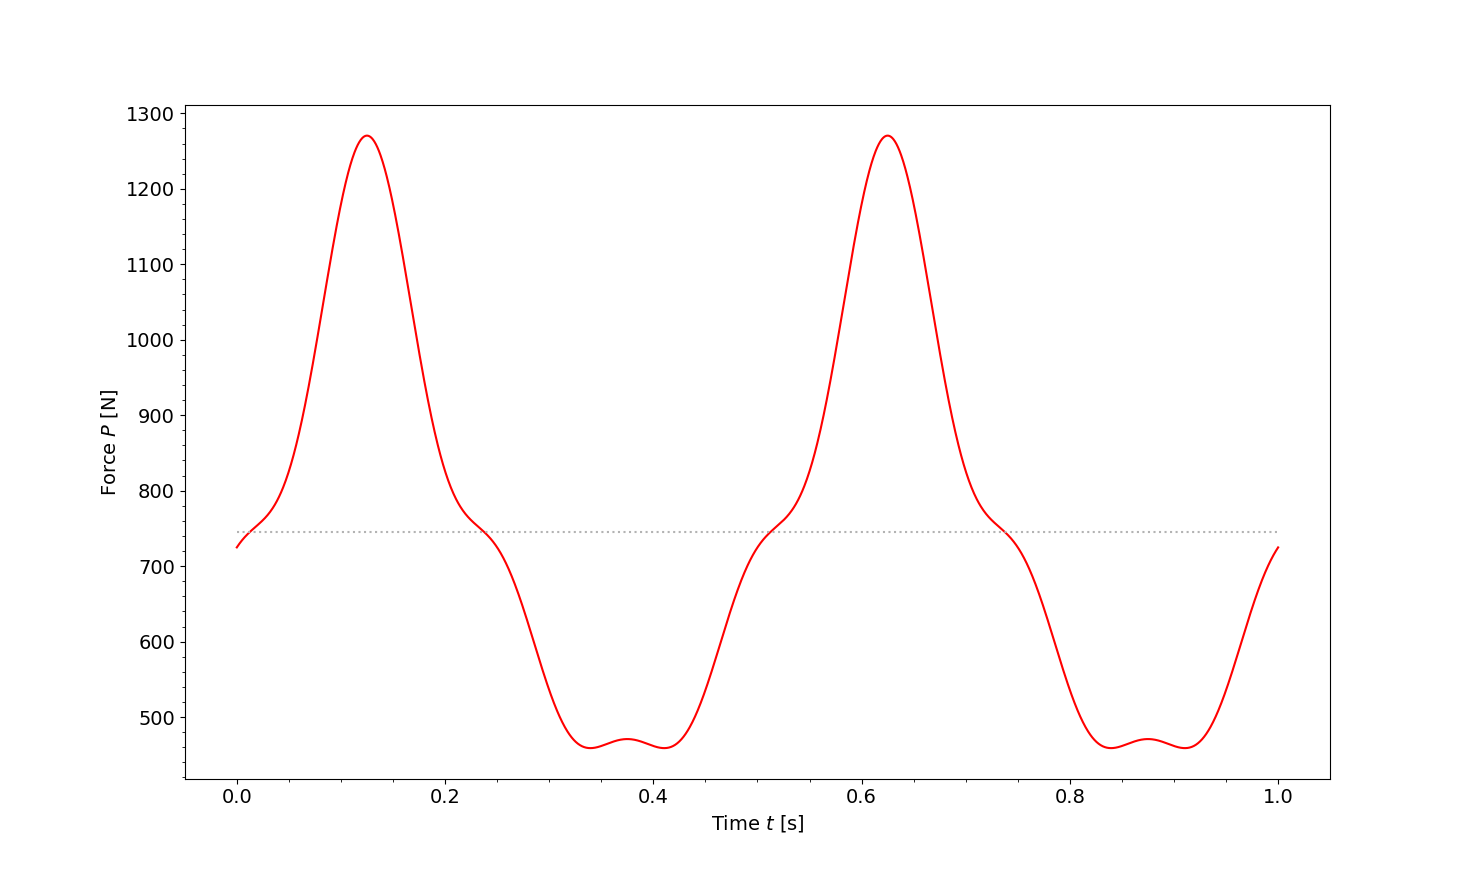
\includegraphics[width=1.0\textwidth]{images/footfall}
\caption{Footfall loading for one walking cycle}
\label{fig:footfall}
\end{figure}

\section{Solution of dynamic response}
\subsection{Theoretical background of modal superposition}
\label{subsec:modal_superposition}
 The equation of motion for a MDOF (multi-degree of freedom) system with damping is
\begin{equation}
\mathbf{m\ddot{u}}+\mathbf{c\dot{u}}+\mathbf{ku}=\mathbf{P}
\label{eqn:motion}
\end{equation}
\noindent
where the square matrices $\textbf{m}$, $\textbf{k}$ and $\textbf{c}$ represent mass, stiffness and damping of the system.

A direct solution of this equation set might be seriously impeded by coupled unknowns, as in normal cases the stiffness matrix $\textbf{k}$ and damping matrix $\textbf{c}$ have off-diagonal terms. The simultaneous solution of these coupled equations is generally not efficient, especially with large amount of DOFs. An alternative is to expand the displacement vector $\mathbf{u}$ of the MDOF system in terms of modal contributions expressed as
\begin{equation}
\mathbf{u}(t)=\sum_{n=1}^N\mathbf{u}_n(t)=\sum_{n=1}^N\boldsymbol{\phi}_nq_n(t)
\label{eqn:u}
\end{equation}
\noindent
where $\boldsymbol{\phi}_n$ is the mode shape and $q_n(t)$ is the associated modal coordinate. Observe that the vibration of each mode is decomposed into two parts, the mode shape that characterizes the vibration pattern along DOFs and keeps invariant to time, the modal coordinate that represents the amplitude of vibration along time points and keeps unchanged for each DOF.  

Using equation \ref{eqn:u}, the coupled equations (\ref{eqn:motion}) can be transformed to a set of uncoupled equations with modal coordinates $q_n(t)$ as the unknowns \cite{chopra2007dynamics}. The equation governs the $n$th modal coordinate $q_n(t)$ reads
\begin{equation}
\ddot{q_n}+2\xi_n\omega_n\dot{q_n}+\omega_n^2q_n=P_n(t)
\label{eqn:motion_q}
\end{equation}
\noindent   
where $\xi_n$ represents the modal damping ratio, $\omega_n$ the angular frequency, $P_n(t)$ the modal load. 

To solve equation \ref{eqn:motion_q}, modal analysis needs to be conducted as the first step for mode shape $\boldsymbol{\phi}_n$ and angular frequency $\omega_n$. They are inherent characteristics of a structure obtained by solving the matrix eigenvalue problem
\begin{equation}
\label{eqn:eigenvalue}
    \left[\textbf{k}-\omega_n^2\textbf{m}\right]\boldsymbol{\phi}_n=\textbf{0}
\end{equation}
\noindent
This equation will have non-trivial solutions only when
\begin{equation}
\label{eqn:eigenvalue_det}
    \text{det}[\textbf{k}-\omega_n^2\textbf m]=0
\end{equation}
\noindent
Through this equation $\omega_n$ can be solved, then substitute the solution in equation \ref{eqn:eigenvalue} to calculate $\boldsymbol{\phi}_n$. Note that the mode shape could be scaled arbitrarily, in this research it is so normalized that the maximum item in each mode is equal to 1. Another modal parameter, modal mass $m_n$, is calculated by
\begin{equation}
\label{eqn:mn}
    m_n = \boldsymbol{\phi}_n^T\textbf{m}\boldsymbol{\phi}_n
\end{equation}

\subsection{Modal analysis}
The mesh models in Rhino, together with information about material, section properties, boundary conditions, the load poin are exported to Abaqus. Abaqus assembles these shell elements and generates the mass matrix and stiffness matrix. The calculation of  modal parameters is based on equation \ref{eqn:eigenvalue} to \ref{eqn:mn}. Figure \ref{fig:mode_shapes} shows the first 4 unique modes (some modes are repeated because of symmetry) of the floor for quick check of the plausibility.
\begin{figure}[H]
\begin{subfigure}[b]{.48\textwidth}
  \centering
  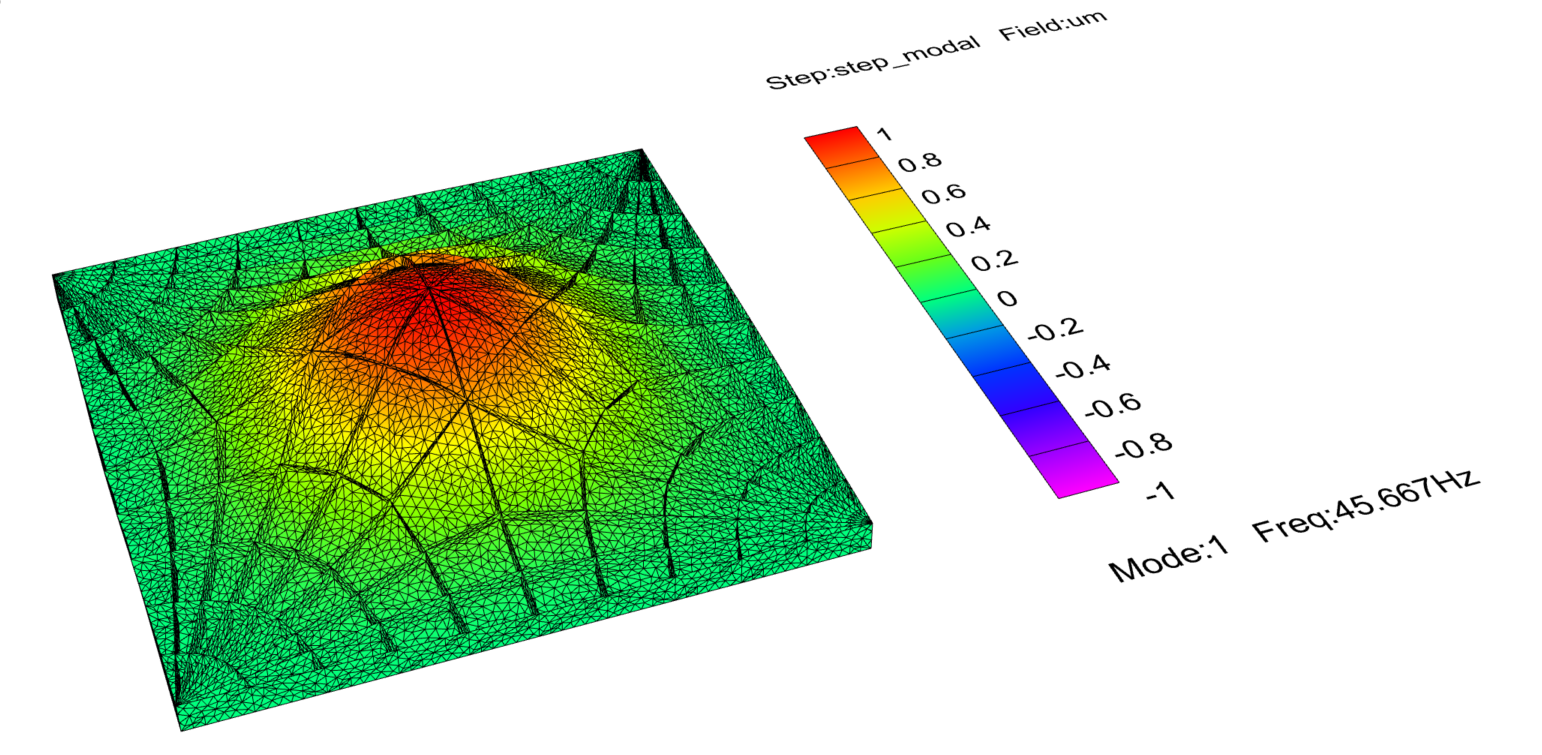
\includegraphics[width=.95\linewidth]{mode1}
  \caption{1st mode}
\end{subfigure}
~
\begin{subfigure}[b]{.48\textwidth}
  \centering
  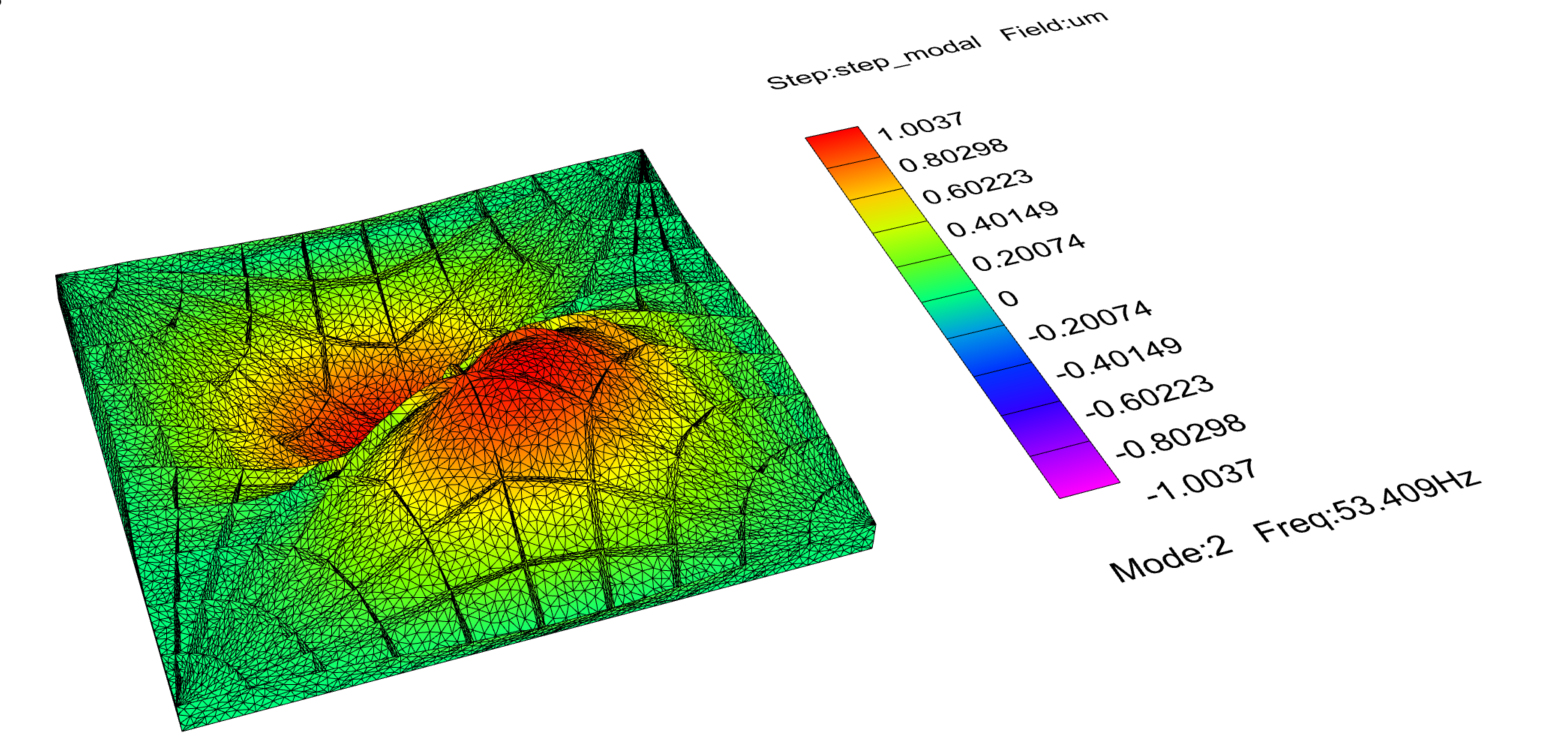
\includegraphics[width=.95\linewidth]{mode2}
  \caption{2nd mode}
\end{subfigure}

\begin{subfigure}[b]{.48\textwidth}
  \centering
  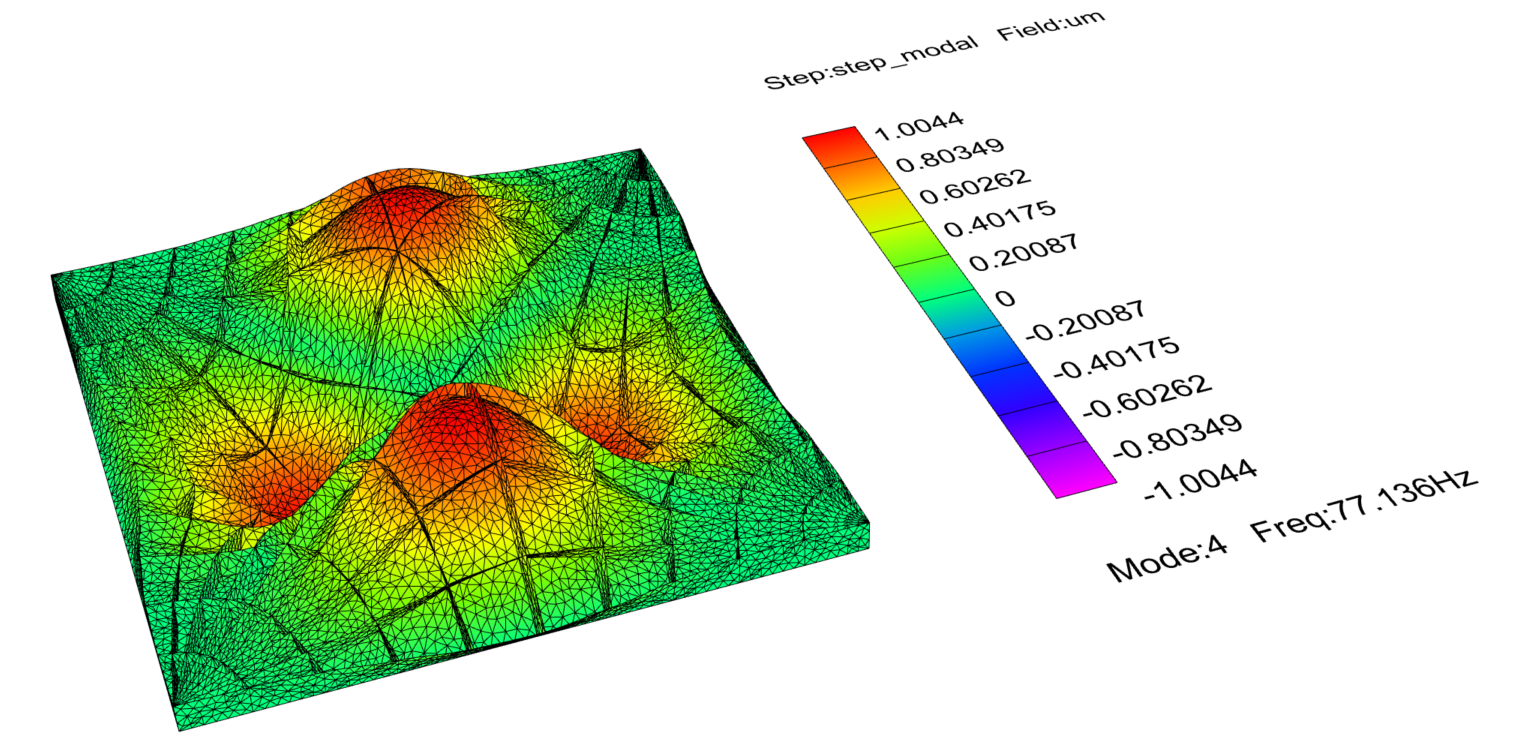
\includegraphics[width=.95\linewidth]{mode4}
  \caption{4th mode}
\end{subfigure}
~
\begin{subfigure}[b]{.48\textwidth}
  \centering
  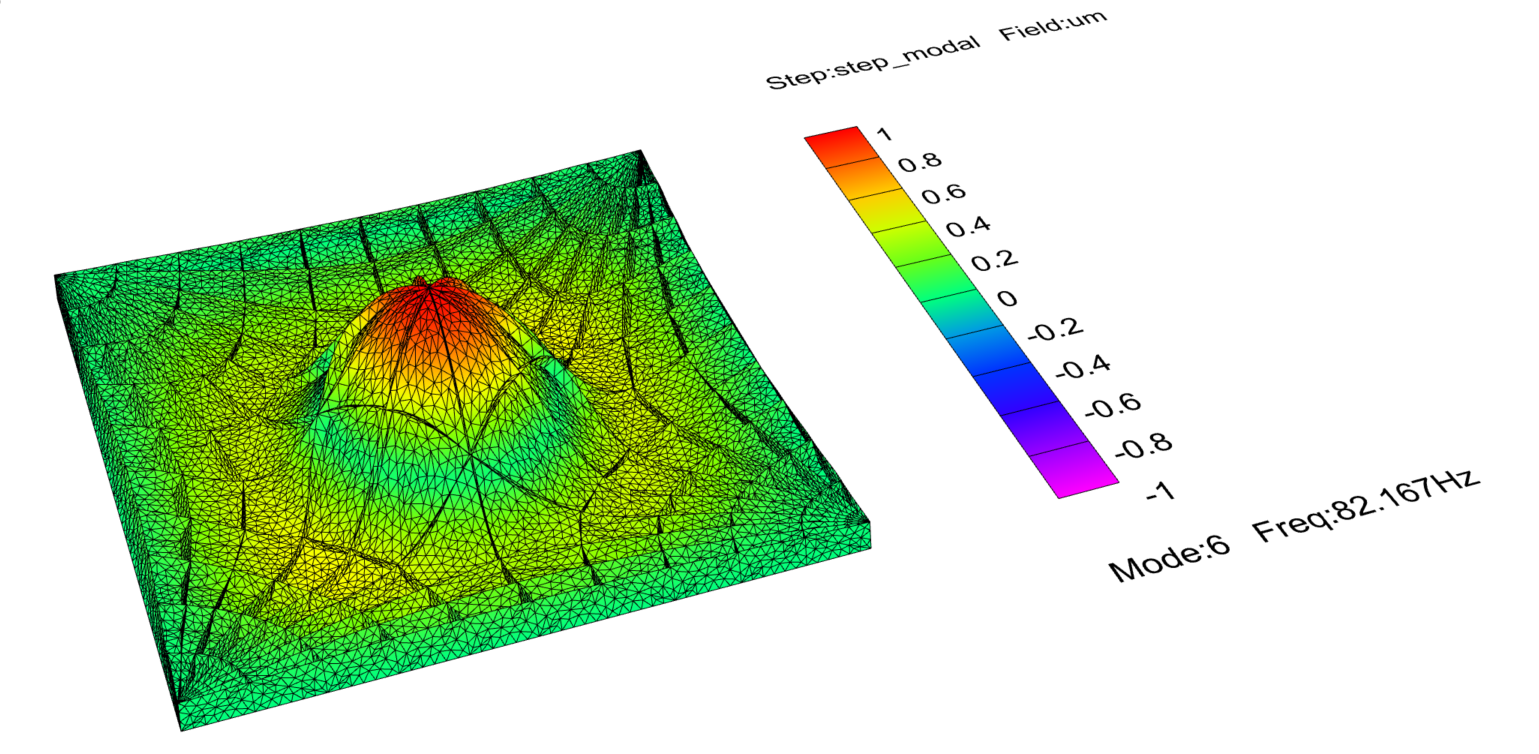
\includegraphics[width=.95\linewidth]{mode6}
  \caption{6th mode}
\end{subfigure}

\caption{The first 4 unique modes of floor with $l=5m, l/d=20, t_v/t_r=1$}
\label{fig:mode_shapes}
\end{figure}


\subsection{Response time history}
\label{subsec:resp_time_histroy}
Since the mode shapes are already available, the next step is to solve the modal coordinates $q_n(t)$ that vary wit time. In equation \ref{eqn:motion_q}, the modal load $P_n(t)$ can be calculated as follows:
\begin{enumerate}
    \item 
     Express the external load $\textbf{P}$(\textbf{s},t) acting on the MDOF system in terms of spatial distribution $\mathbf{s}$ and time variation $P(t)$: 
    \begin{equation}
    \mathbf{P}(\mathbf{s},t)=\mathbf{s}P(t)
    \end{equation}
    \noindent
    where spatical distribution \textbf{s} is a vector of size the number of DOFs in the system, with representative value in position whose corresponding DOF is loaded, and with 0 if not loaded. Time variation $P(t)$ can be the footfall loading expressed in equation \ref{eqn:footfall_SCI}. 

    \item
    Calculate the modal participation factor 
    \begin{equation}
    \label{eqn:Gamma}
    \Gamma_n=\frac{\boldsymbol{\phi}_n^T\mathbf{s}}{M_n}
    \end{equation}
    
    \item
    Then modal load
    \begin{equation}
    P_n(t)=\Gamma_nP(t)
    \end{equation}
\end{enumerate}

Once the modal load is obtained, the second order, ordinary differential equation (\ref{eqn:motion_q}) can be reformed into two first order, ordinary differential equations, expressed in matrix form
\begin{equation}
\begin{bmatrix} \dot{q_n}\\ \ddot{q_n} \end{bmatrix} 
=\begin{bmatrix} 0 & 1 \\ -\omega_n^2 & -2\xi_n\omega_n \end{bmatrix}
\begin{bmatrix} q_n\\ \dot{q_n} \end{bmatrix}
+ \begin{bmatrix} 0\\ P_n(t) \end{bmatrix}
\end{equation}
\noindent
This matrix equation can be solved with the ODE solver \textit{odeint} in the SciPy module.  Two initial conditions at $t=0$ that represent a rest state, initial displacements $q_n(0)=0$ and initial velocity $\dot{q_n}(0)=0$, are assumed. The results of the \textit{odeint} solver are the displacements and velocities in modal coordinates. The accelerations are then calculated by differentiating the velocities with respect to time. Once the modal coordinates $q_n(t)$ have been solved, the total displacements can be obtained via modal superposition expressed in equation (\ref{eqn:u}).

\section{Evaluation of vibration perception}
The evaluation of the dynamic performance is based on the vibration perception of humans, which is characterized by the frequency weighted root-mean-square (RMS) acceleration of the floor under the footfall loading, expressed by 
\begin{equation}
\label{eqn:aw_rms}
    a_{w,rms}(t)=\sqrt{\frac{1}{T}\int_0^Ta_w(t)^2dt}
\end{equation}
\noindent
where $T$ is the period under consideration, taken as $1/f_p$. The frequency weighted total acceleration $a_w(t)$ is found by summing the acceleration responses of each mode
\begin{equation}
    a_w(t)=\sum_{n=1}^Na_{n,w}(t)
\end{equation}
\noindent
The vibration perception of humans is different with varying vibration frequencies. Humans are generally not sensitive to vibrations with too low or too high frequencies, so actual acceleration should be weighted to reflect the perception of humans. Figure \ref{fig:Wb} shows the frequency weighting curve and functions for vertical vibrations recommended by SCI P354. The weighted acceleration then reads
\begin{equation}
    a_{n,w}(t)=W_b(f_n)a_n(t)
\end{equation}
\noindent
where $a_n(t)$ is the actual acceleration in each mode solved by response time history analysis.

\begin{figure}[H]
\begin{subfigure}[H]{.48\textwidth}
  \centering
  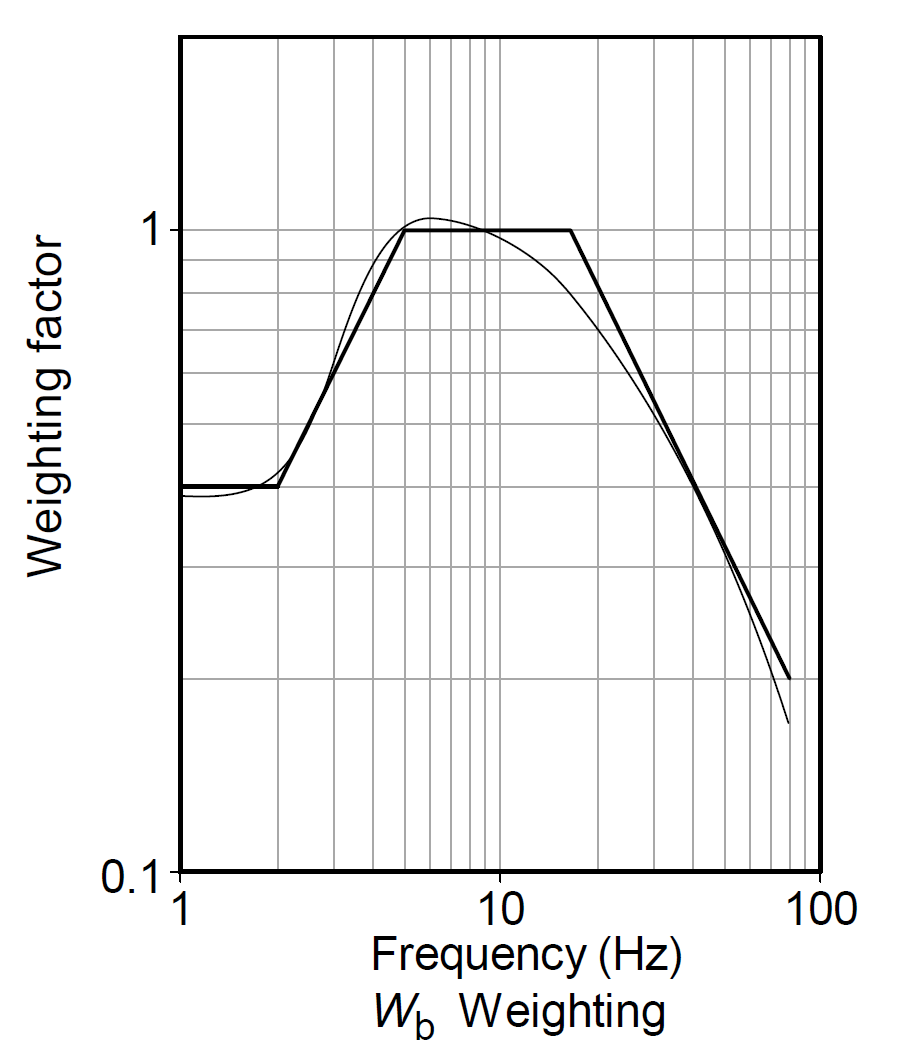
\includegraphics[width=.95\linewidth]{weight_curve}
\end{subfigure}
~
\begin{subfigure}[H]{.5\textwidth}
  \centering
  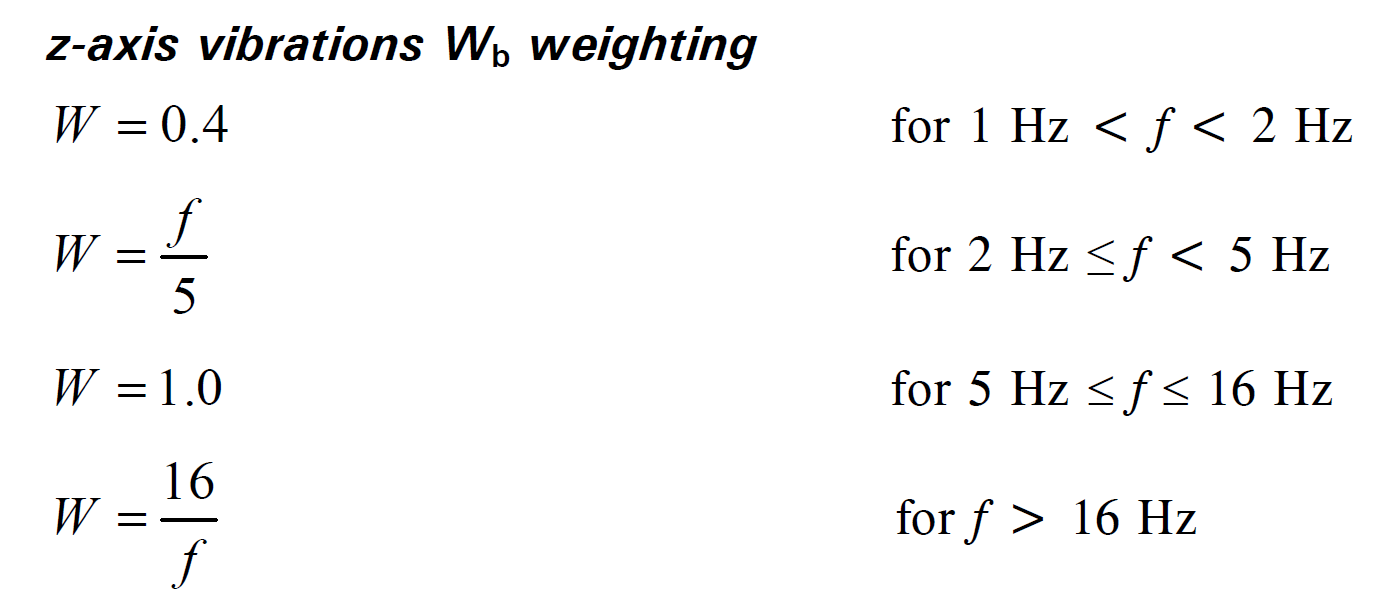
\includegraphics[width=.99\linewidth]{weight_fn}
\end{subfigure}

\caption{Frequency weighting $W_b$}
\label{fig:Wb}
\end{figure}

The next step is to calculate the response factor, which is the ratio between the weighted rms-acceleration $a_{w,rms}$ (peak value) calculated by equation \ref{eqn:aw_rms} and the base value $a_{rms,base}=5\times10^{-3}$ m/s\textsuperscript{2}.

\begin{equation}
    R=\frac{a_{w,rms}}{a_{base,rms}}=\frac{a_{w,rms}}{0.005}
\end{equation}

The response factor should not exceed the recommended multiplying factors listed in table \ref{table:multiplier_SCI}. For office buildings, the maximal response factor is 8, meaning that the allowable weighted rms-acceleration $a_{w,rms,allow}=0.04$\,m/s\textsuperscript{2}.
\begin{table}[H]
\centering
\caption{Recommended multiplying factors based on single person excitation}
\label{table:multiplier_SCI}
\begin{tabular}{c}
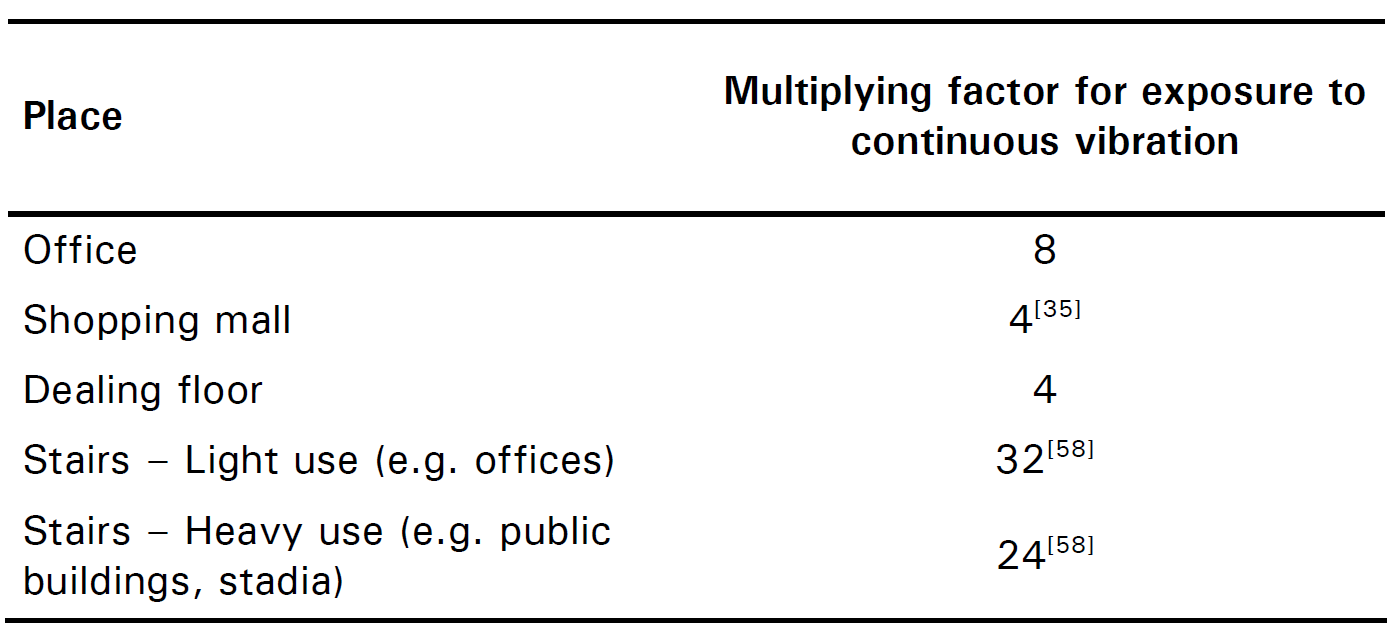
\includegraphics[width=0.7\textwidth]{multiplier_SCI}
\end{tabular}
\end{table}